\section{Role Based Access Control Standard} \label{sec:core-rbac}

RBAC provides effective and efficient permissions management for operations, especially when sharing resources within an organization.
Prior to the creation of the NIST RBAC standard, no general agreement on the definition 
of RBAC existed among practitioners or within the research community. 
Without a unified definition of RBAC, software developers described similar concepts and features of RBAC models using different terminology. 
This lack of consistent terminology was shown to slow the implementation of RBAC \cite{o20102010}.  
Moreover, in cases where organizations were concerned with adopting RBAC,
evaluation and comparison of RBAC technologies developed by different vendors was difficult.
NIST, in collaboration with industry and academics, worked on defining a set of consensus RBAC concepts and terminology and proposed a standard for 
RBAC that addressed these cost and interoperability issues by developing a common definition that can be used across different vendors.

NIST's work can directly benefit organizations by lowering cost of early phase R\&D and the implementation of RBAC.
Since the RBAC standard was first introduced, a 2010 report by RTI International showed that the the rate of RBAC adoption has rapidly grown over recent years \cite{o20102010}. 
The analysts estimate that, by the end of 2010, at least a part of permission of systems use RBAC for more than 50\% of IT users at organizations, which
hire more than 500 employees. For economic estimate analysis, the analysts estimate that RBAC technology has generated \$6.1 billion in net economic benefits to industry, of which \$1.1 billion is attributable to NIST RBAC standard work.

The NIST RBAC standard model proposed by Ferraiolo et al. \cite{ferraiolo} and later adopted as the official standard for RBAC by the INCITS includes three levels of RBAC: core RBAC, hierarchical RBAC, and constrained RBAC.
Since the basis for our review is extensions to the RBAC standard model, we describe the core model, associated entities and other terminology encountered across the space of our review. Then, we describe hierarchical RBAC and constrained RBAC, which are developed by incorporating new features into the core RBAC. 

\subsection{Core RBAC} 

The four entities of the standard RBAC model are:

\begin{itemize}
\setlength{\itemsep}{0.25pt}
\item a set of \emph{Users}: A user can be a person or an agent.
\item a set of \emph{Roles}: A role is a collection of permissions to perform a specific job function in an organization.
\item a set of \emph{Permissions}: A permission refers to an access mode that can be exercised on an object in the system and a session relates a user to possibly many roles.
\item a set of \emph{Sessions}: In each session, a user can be assigned to some of the roles, only when the corresponding role is enabled for activation for that time.		
\end{itemize}

In RBAC, a user can exercise a permission only if the user is assigned to a role.
In addition to the four basic components, two functions are defined:
the user role assignment (UA) and the role and permission assignment (PA) functions.
User role assignment models assignment of users to roles.
Permission role assignment models assignment of permissions to roles.

\begin{figure}[ht]
    \centering
        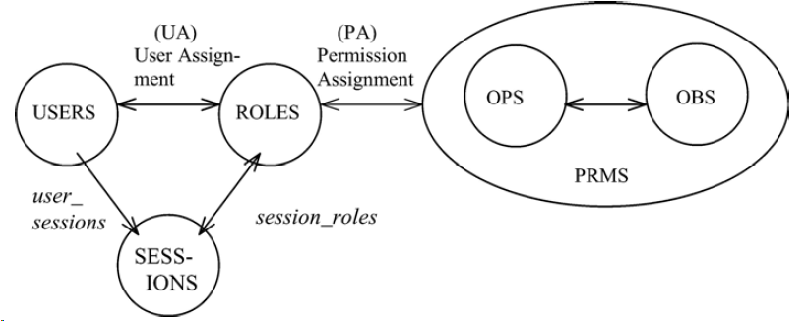
\includegraphics[width=4.0in]{sections/core-model.png}
    \caption{\label{fig:overview}RBAC Core Diagram in NIST RBAC model \cite{ferraiolokuhn}.}
\end{figure}

Figure~\ref{fig:overview} presents an overview of core RBAC model diagram where elements and their relations are described.
Let "USERS", "ROLES", "OBS", "OPS", "PRM", and "SESSIONS" denote users, roles, objects, operations, permissions, and sessions, respectively.
Permissions are associated with possible users' pre-defined operation on an object (e.g., execute a file).
Note that, at user or role activation, a session associated with user or role is established.

\subsection{Hierarchical RBAC} 

Hierarchical RBAC model adds role hierarchies (RH) feature to core RBAC model.
This model incorporates a structure of roles in an organization using inheritance relationship among attributes such as roles.
The role structure in an organization may use
a role $r_1$, who inherits all permissions of another role $r_2$.
For example, a manager role may inherit all permissions of a employee role.
Role hierarchies help simplify access control policy creation and maintenance by reducing the number of
individual role assignments to a user. Formally, role inheritance relation is shown as \textit{RH} $\subseteq$ \textit{ROLES} $\times$ \textit{ROLES} describing many-to-many mapping role inheritance relation. 
General role hierarchies can be extended to use the concept of multiple inheritance where
a role $r_1$, who inherits all permissions from more than one roles.


\subsection{Constrained RBAC}

Constrained RBAC incorporates static and dynamic separation of duty relations to the RBAC model. Separation of 
duty relations enforce conflict of interest among roles. This model defines two types of separation of duty relations; static and dynamic.

\begin{itemize}
	\item Static Separation of Duty (SSoD): SSoD restricts the conflicting-role assignments statically that are associated with a user. On situations
	where multiple roles can be associated with a single user and roles $Role_A$ and $Role_B$ are conflicting each other, no permission is given to a user who is assigned to both $Role_A$ and $Role_B$. SSoD is known to be too rigid for practical use in cases where a user should have permissions as either $Role_A$ and $Role_B$.
	\item Dynamic Separation of Duty (DSD): Dynamic SoD is known to be
more flexible than SSD. DSD restricts the conflicting-role assignments dynamically that are associated with a user. On situations
	where multiple roles can be associated with a single user and , given a context, roles $Role_A$ and $Role_B$ are conflicting each other dynamically, no permission is given to a user.	
\end{itemize}
